\documentclass[final,5p,times]{elsarticle}  % Uncomment for final style formatting
%\documentclass[review,times]{elsarticle}  % Uncomment for review/manuscript style formatting

\usepackage{graphicx} % Required for inserting images
\usepackage{lineno,hyperref}
\usepackage{diagbox}
\usepackage{xcolor}
\modulolinenumbers[5]

\journal{}

% \bibliographystyle{elsarticle-num}  %% `Elsevier LaTeX' style
% \bibliographystyle{elsarticle-num_etal}  % author lists shortened
% \bibliographystyle{elsarticle-num_etal_no_doi}  % author lists shortened and DOI hidden
\bibliographystyle{elsarticle-num_etal_title_no_extra_url.bst} % first author et al, title with link, no extra url

\usepackage{dcolumn}% Align table columns on decimal point
\usepackage{bm}% bold math

\usepackage[utf8]{inputenc}
\usepackage[T1]{fontenc}
\usepackage{mathptmx}
\usepackage{mathtools}
\usepackage{etoolbox}
\usepackage{hyperref}
\usepackage{textcomp}

\usepackage{acro}
\DeclareAcronym{2PM}{short=2PM,long=2-Point Model}
\DeclareAcronym{3LP}{short=3LP,long=triple-tipped Langmuir probe}
\DeclareAcronym{Afrac}{short=$A_{frac}$, long=attachment fraction}
\DeclareAcronym{afrac}{
    short=$J_{sat}/J_{roll}$,
    long=\ac{Jsat} normalized to its value at rollover
}
\DeclareAcronym{CLTF}{short=CLTF,long=closed loop transfer function}
\DeclareAcronym{DTS}{short=DTS, long=Divertor Thomson Scattering}
\DeclareAcronym{FOPDT}{short=FOPDT,long=First Order Plus Dead Time}
\DeclareAcronym{GGD}{short=GGD, long=Generalized Grid Description}
\DeclareAcronym{IDS}{short=IDS, long=Interface Data Structure}
\DeclareAcronym{IMAS}{short=IMAS, long=ITER Integrated Modelling and Analysis Suite}
\DeclareAcronym{IRVB}{short=IRVB, long=Infra-Red Video Bolometer}
\DeclareAcronym{ITB}{short=ITB, long=Internal Transport Barrier}
\DeclareAcronym{ITER}{short=ITER, long=International Thermonuclear Experimental Reactor}
\DeclareAcronym{Jsat}{short=$J_{sat}$,long=ion saturation current density}
\DeclareAcronym{LCFS}{short=LCFS, long={Last Closed Flux Surface}}
\DeclareAcronym{LP}{short=LP,long=Langmuir probe}
\DeclareAcronym{MIMO}{short=MIMO, long={multi in, multi out}}
\DeclareAcronym{MPC}{short=MPC, long=Model Predictive Control}
\DeclareAcronym{NBI}{short=NBI, long=neutral beam injection}
\DeclareAcronym{OLTF}{short=OLTF,long=open loop transfer function}
\DeclareAcronym{OSP}{short=OSP, long=outer strike point}
\DeclareAcronym{PCS}{short=PCS,long=plasma control system}
\DeclareAcronym{PFR}{short=PFR,long=private flux region}
\DeclareAcronym{PID}{short=PID,long=proportional-integral-derivative}
\DeclareAcronym{Prad}{short=$P_{rad}$,long=radiated power}
\DeclareAcronym{Pradcore}{short=$P_{rad,core}$,long=core radiated power}
\DeclareAcronym{PSOL}{short=$P_{SOL}$, long=power crossing into the scrape-off layer}
\DeclareAcronym{PVLC}{short=PVLC, long=Predicted Variable Linear Controller}
\DeclareAcronym{RT}{short=RT, long=real-time}
\DeclareAcronym{SISO}{short=SISO, long={single in, single out}}
\DeclareAcronym{SOPDT}{short=SOPDT,long=Second Order Plus Dead Time}
\DeclareAcronym{SOL}{short=SOL, long=Scrape-off Layer}
\DeclareAcronym{SOLPS-ITER}{short=SOLPS-ITER, long=Scrape-off Layer Plasma Simulator - ITER version}
\DeclareAcronym{UGF}{short=UGF, long=unity gain frequency}
\DeclareAcronym{ZN}{short=Z-N, long=Ziegler-Nichols}
\providecommand{\acroifusedTF}{\acifused}

% New command for citation reminder
\newcommand{\needcite}{\textbf{ [NEEDCITE]}}

% New command for possible changes in wording
\newcommand{\maybe}[1]{\textcolor{red}{(or #1)}}

\newcommand{\Afrac}{A$_{frac}$\ }

% Recoloring links for figures and citations makes the draft easier to read than having the colored boxes around things. Won't matter in the final; the published version always is cleaned up. But this is nice for the manuscript.
\hypersetup{colorlinks,linkcolor={red!50!black},citecolor={green!50!black}, urlcolor={blue!50!black}}

% Institution shortcuts
\def\GApo{General Atomics, PO Box 85608, San Diego, CA 92186-5608, USA}
\def\GA{General Atomics, 3550 General Atomics Ct., San Diego, CA 92121, USA}
\def\ORAU{Oak Ridge Associated Universities, 100 ORAU Way, Oak Ridge, TN 37830, USA}
\def\ORNL{Oak Ridge National Laboratory, Oak Ridge, TN 37831, USA}
\def\SNL{Sandia National Laboratories, Livermore, CA, 94550, USA}
\def\LLNL{Lawrence Livermore National Laboratory, PO Box 808, Livermore, CA 94550, USA}
\def\PPPL{Princeton Plasma Physics Laboratory, P.O. Box 451, Princeton, NJ 08543-0451, USA}
\def\Princeton{Princeton University, Princeton, NJ 08544, USA}
\def\Wisc{University of Wisconsin - Madison, Madison, WI 53706, USA}
\def\UCSD{University of California - San Diego, San Diego, CA 92093, USA}
\def\MIT{Massachusetts Institute of Technology, 77 Massachusetts Ave, Cambridge, MA 02139, USA}
\def\Eindhoven{Eindhoven University of Technology, Eindhoven, 5612 AZ, The Netherlands}
\def\York{University of York, Heslington, York YO10 5DD, United Kingdom}
\def\ASIPP{Institute of Plasma Physics, Chinese Academy of Sciences, Hefei 230031, China}
\def\CCFE{Culham Centre for Fusion Energy, %Culham Science Centre, 
Abingdon OX14 3EB, United Kingdom}
\def\KFE{Korea Institute of Fusion Energy, 169-148 Gwahak-ro, Yuseong-gu, Daejeon 34133, Republic of Korea}
\def\UTK{University of Tennessee-Knoxville, Knoxville, TN 37996, USA}
\def\Columbia{Columbia University, 116th and Broadway, New York, NY 10027, USA}

\begin{document}

\title{Detachment control in KSTAR with Tungsten divertor}
\author[ORAU]{Anchal Gupta\corref{mycorrespondingauthor}}
\cortext[mycorrespondingauthor]{Corresponding author}
\ead{guptaa@fusion.gat.com}

\author[GA]{David Eldon}

\author[ORAU]{KyuBeen Kwon}

\author[GA]{Anthony Leonard}

\author[LLNL]{Xueqiao Xu}

\author[LLNL]{Menglong Zhao}

\author[LLNL]{Ben Zhu}

\address[ORAU]{\ORAU}
\address[GA]{\GA}
\address[LLNL]{\LLNL}

\date{\today}

\begin{abstract}
KSTAR has recently undergone an upgrade to use a new Tungsten divertor to run experiments in ITER-relevant scenarios.
Even with a high melting point of Tungsten, it is important to control the heat flux impinging on tungsten divertor targets to minimize sputtering and contamination of the core plasma.
Heat flux on the divertor is often controlled by increasing the detachment of \ac{SOL} plasma from the target plates.
In this work, we have demonstrated successful detachment control experiments using two different methods.
The first method uses attachment fraction as a control variable which is estimated using ion saturation current measurements by embedded Langmuir probes in the divertor.
The second method uses a novel machine-learning-based surrogate model of 2D UEDGE simulation database, DivControlNN.
We demonstrated running inference operation of DivControlNN in realtime to estimate heat flux at the divertor and use it to feedback impurity gas to control the detachment level.
We present interesting insights from these experiments including a systematic approach to tuning controllers and discuss future improvements in the control infrastructure and control variables for future burning plasma experiments.
\end{abstract}

\acresetall  % Reset acronyms after the abstract. This has unexpected behavior for acronyms that aren't used later.

\maketitle


\section{Introduction}
\label{sec:introduction}

Burning plasma tokamaks such asITER\cite{Holtkamp_2007_FED}, SPARC\cite{Creely_2020_JPP}, and the various DEMO concepts are estimated to exhaust very high heat flux in the \ac{SOL} towards the divertor. Significant research has been carried over designing such divertors to withstand the high heat flux and ITER project has decided to use Tungsten as the divertor material. Thus, experimental reactors such KSTAR are in the process of upgrading their divertor and vessel walls to tungsten to design control systems with tungsten present in the vessel and perform plasma study experiments with tunsgten contamination. Even with high melting point of tungsten, it is estimated that perpendicular heat flux on the divertor should be limited to 10--15~MW~$\mathrm{m}^{-2}$\cite{pitts_2019_nme} and the electron temperature at the divertor should remain within 8 eV\cite{Brezinsek_2019_NF} to avoid sputtering of tungsten and subsequent contamination of core plasma.

The heat flux reaching the divertor is typically reduced by puffing in impurity gases to dissipate energy and momemntum of the plasma in \ac{SOL} region. However, excessive impurity seeding could result in core contamination which not only reduces the fusion yield but can also cause cooling of core plasma resulting in collapse of H-mode or disruption in some cases. Thus, it is important to carefully control the amount of impurity injected to keep the divertor cool while not contaminating the core plasma. This control is generally referred as detachment control as the divertor leg is detached from the divertor target leg and controlled to a specific level of detachment.

Several successful attempts at controlling detachment levels in experimental reactors have been achieved with various impurity gases\cite{Kallenbach_2012_NF,Ravensbergen_2021_NC, Eldon_2022_PPCF}. These experiments were not conducted in tungsten divertor conditions though, where contamination from tungsten can potential cause issues in the control technique. In this work, we demonstrated detachment control in KSTAR 2024 experimental campaign where a tungsten divertor was installed.

This paper is organized as following. In Sec.\ref{sec:control_variables}, we describe the experimental setup and the definition of different control variables used for detachment control. In Sec.\ref{sec:sysid}, we describe our experimental shots used for identifying the system and using the fitted plant model to tune a PI controller using frequency response for closed-loop stability analysis and optimization. In Sec.\ref{sec:results}, we show the results of our detachment control attempts. And finally, in Sec.\ref{sec:discussion}, we discuss our results, the possible improvements we can make in future, and other interesting contemporary work and ideas in the field of detachment control.

\begin{figure}[!ht]
 \centering
 \includegraphics[width=\linewidth]{figures/RefShot_35851.pdf}
 \caption{
Reference shot \#35851.
(a) Showing last closed flux surface (solid blue) and the secondary separatrix (dotted blue) at t=8 seconds.
The magnetic shape control was programmed to keep X point fixed which provided a sufficiently stable strike point on the realtime \ac{LP} array.
(b) Zoomed-in locations of realtime Outer Divertor (OD) \acp{LP}.
(c) Plasma current (I$_p$) and $\beta_n$ for reference shot.
}
 \label{fig:ref_shot}
\end{figure}
% Consider adding a contour for the secondary separatrix (I typically have to guess and check psi_N values until I find the one that makes another X). The modelers usually like this. If you decide to include this, make the secondary contour a lighter weight than the primary.
% It may be of some minor interest to include a thin or dashed outline of the former carbon limiting surface, which I think would be purely outboard of the tungsten surface and therefore not too confusing. However, this could be too busy and I'm not sure it should go in the final. Just something to think about.

\section{Experimental setup and control variables}
\label{sec:control_variables}

\begin{figure}[!ht]
 \centering
 \includegraphics[width=\linewidth]{figures/StrikePointWidth.pdf}
 \caption{
Strike point width estimation for reference shot \#35851.
The raw data from langmuir probe array has been filtered by 4th order Butterworth filter with cut-off frequency of 20 Hz and then down sampled to 40 Hz.
For each data point on this plot, the x-axis position is calculated by subtracting the \ac{OSP} position reported by EFIT from the probe's Z coordinate.
The black dotted lines represent the rough estimate for width of strike point ion saturation current profile taken at half the maximum value above baseline.
}
 \label{fig:strike_point_width}
\end{figure}

The experiment was conducted on a standard lower single null H-mode plasma profile with reference shot KSTAR \#35851 with the equilibrium profile as shown in Fig.\ref{fig:ref_shot}.
The plasma shaping steps commenced by 7~s and the shot was programmed for flat-top up to 17~s providing a 10~s long window for the detachment control experiment.
For heat flux control, N$_2$ gas puffing was used.
The heat flux control variable was tested with several different inputs.

First, we utilized previously developed \ac{Afrac} \cite{Eldon_2022_PPCF}, which is defined as the ratio of measured ion saturation current ($I_{sat, measured}$) to modeled (using 2PM \cite{Leonard_2018_PPCF}) ion saturation current assuming fully attachment plasma ($I_{sat, attached}$).
\begin{equation}
    A_{frac} = \frac{I_{sat, measured}}{I_{sat, attached}}
\end{equation}

$I_{sat, attached}$ is estimated using Eq.(13) from \cite{Eldon_2022_PPCF}:

\begin{equation}
    I_{sat, attached} = C \langle n_{e} \rangle^2 q_{||, a}^{-\frac{3}{7}} 
\end{equation}

Here, $C$ is a calibration constant determined during reference shots so that \ac{Afrac} is 1.0 when \ac{SOL} plasma is fully attached to the divertor, $\langle n_{e} \rangle$ is the line-averaged electron density measured by interferometer and $q_{||, a}$ is the heat flux density at the outer mid-plane which is estimated using Eq.(15) from \cite{Eldon_2022_PPCF}.
The calibration constant $C$ accounts for gaps in real-time data availability on KSTAR and may be removed if more measurements become available in the future.
\ac{Afrac} is a convenient choice of control variable that is easily available in most tokamaks and allows for cross-comparison among machines.
If the strike point on the divertor tile is fixed in position well enough by the shape control system, a single close-by Langmuir probe is enough to provide the ion saturation current required for \ac{Afrac} calculation.
However, if the strike point control is not good enough, or if it is required to leave it as a free variable to allow for controlling other parameters in the shape control loop (as was the case in our experiments), then it is required to estimate the true ion saturation current through measurements made by a Langmuir probe array.
In our experiments, we chose the peak value from the Langmuir probe array as the input to the ion saturation current at the strike point.
Fig.\ref{fig:strike_point_width} plots the data from this Langmuir probe array for our reference shot.
The horizontal axis in this figure has been referenced from the EFIT reported \ac{OSP} position.
Thus, this figure shows the spread of the ion saturation current profile across the strike point.
Here, we see that the strike point is closer to OD8 and OD9 with a peak ion saturation current value of roughly 0.2~A at the strike point position.
We estimate the width of the ion saturation current profile at half the maximum value referenced to the baseline value of 0.05~A measured by far away probes, giving FWHM$\gtrsim$16~mm.
This ensures that when the strike point is within the closely placed probes, OD8, OD9, and OD11 (Fig.\ref{fig:ref_shot}), at least one probe can measure the ion saturation current while being within the peak region of the strike point.
We used the maximum value measured among the probe array to calculate \ac{Afrac} and since these probes are 12.5~mm apart, it means that the maximum deviation from the actual peak value would be $\lesssim$35\%.
Assuming that the strike point stays for equal amount of time in any location between the probe array (uniformly distributed, this can be further corraborated by noticing the motion of strike point in the figures in later sections), the mean error in peak value would be about 13\% while median error would be about 10\% assuming a gaussian profile with 16~mm FWHM.
This estimation in turn sets goals for a potential future strike point controller, to bound the strike point movement within 6.25~mm of the probe location to achieve above mentioned uncertainties.
If such a strike point controller can keep the strike point motion within 2.35~mm, the mean error would go below 2\% which would already be better than the other sources of error in the ion saturation current measurement.

Langmuir probes would not be able to survive high heat flux in burning plasma future reactors.
In general, such reactors would be severely limited in the number of real-time sensors available for control systems because of high neutron fluence and heat flux in vacuum vessels, and thus alternate control variables need to be searched for.
Toward this goal, we tested a prototype of a machine-learning-based surrogate model of 2D UEDGE, DivControlNN.
The employed version of DivControlNN is trained on approximately 70,000 2D UEDGE simulations of KSTAR.
The training dataset scanned core electron density ($1.5 \times 10^{19} - 7.0 \times 10^{19}$ m$^{-3}$), plasma current ($600-800$ kA), total input power split evenly between ion and electron channels ($1-8$ MW), impurity fraction with respect to Deuterium density ($0-0.04$), and scaling of diffusion coefficient profile with a factor ($0.6 - 2$).
The diffusion coefficient profile is assumed for a typical H-mode shot which can be scaled as an input to the model.
This provided a widely applicable surrogate model that gives steady-state values of heat flux, ion saturation current, and electron temperature along the two divertors, electron density and temperature at the upstream point of the midplane, and total radiated power, power fraction radiated from divertor, and peak radiation power location in the poloidal cross-section of the device.
Values are relative to local profiles (peaks) or relative to magnetic geometry (1D profiles could be extracted, or values at the separatrix), so minor deviations to the plasma boundary shape are likely to be minor sources of error.
Even larger departures from the model plasma shape will not cause errors directly due to mis-mapping positions, although other plasma behaviors would be expected to have some sensitivity to boundary shape.
The model generates output within 20\% error from the 2D UEDGE output.

The model runs in the UEDGE database are all converged to steady state, yet we are operating a controller that deals with plasma dynamics.
The reason we propose this is acceptable is because the model is being used to relate upstream conditions to divertor conditions, and the timescale of the SOL is very fast: we would expect most changes to the SOL to propagate at the ion acoustic speed $c_s$ and thus equilibrate much faster than any other timescale in the problem.
For example, in deuterium plasma at 40~eV (half of the typical $\sim80$~eV separatrix $T_e$ estimate for mid-sized tokamaks like \mbox{DIII-D} and KSTAR \cite{stangeby_2015_nf}), $c_s=391$~km$\;$s$^{-1}$.
For a 30~m connection length that might be reasonably found in the near SOL of KSTAR, communication between the midplane and divertor would take place on timescales of about 80~$\mu$s.
This is twice as fast as the DivControlNN computation time, so modeling the SOL as steady state is not a significant source of error.
There could be issues with the part of the UEDGE model that is within the separatrix, and with properly accounting time between power being injected into the core and it flowing into the UEDGE mesh, and treatment of these should be refined as development progresses.

DivControlNN is not expected to be able to properly describe the plasma state during an ELM or other fast transient event.
This is of no great concern as controlling detachment with gas during ELMs is both impossible (they are much faster than the gas system can respond) and unnecessary (ELMs must be eliminated in reactor class device to allow adequate longevity of plasma facing components), so we must only find a reasonable way to ignore ELMs as has been done with other detachment controllers \cite{Eldon_2017_NF,Eldon_2021_NME}.
As none of the inputs to DivControlNN---input power, plasma current, line-average density, assumed diffusion coefficients, and estimated impurity concentration*---are very sensitive to ELMs, the model effectively ignores ELMs and should function similarly to other control signals where more effort has been made to suppress perturbations due to ELMs.
Particularly large ELMs could show as dips in average density and indeed produce a noticeable cycle of pedestal regrowth after each ELM crash, but this scenario did not produce ELMs this large and it was not necessary to treat a pedestal recovery cycle yet.

DivControlNN was originally developed and trained using Python's TensorFlow package and consists of two different models working in tandem.
The first is a multi-modal $\beta$-variational autoencoder \cite{Higgins_2017_ICLR} model to compress various quantities of interest coming from synthetic diagnostics on a 2D UEDGE database into a latent space representation.
The second stage is a multi-layer perceptron (MLP) model that maps the inputs of the 2D UEDGE simulations (which also form the inputs to the overall surrogate model).
During inference operation, the MLP model first maps the inputs to the latent space and the decoder network from the autoencoder then decodes the latent space into useful outputs.
While Python is the industry choice for developing and training such models, it can not be used for real-time inference purposes such as our use case.
We converted the Python model into a pure C code using a \texttt{keras2c} \cite{keras2c} package which is developed for generally converting such neural networks into real-time compatible C codes.
The generated C code runs an inference operation in about 160 $\mu$s on Intel\textsuperscript{\textregistered} Core\textsuperscript{TM} i7-6600U CPU @ 2.60GHz while we saw speed up of up to 18~$\mu$s per inference on Apple\textsuperscript{\textregistered} M2\textsuperscript{TM} Pro.
The real-time PCS in KSTAR runs its divertor control categories in a 50~$\mu$s clock cycle CPU, so we ran DivControlNN in a separate 1~ms clock-cycle CPU ensuring enough runtime for it along with other processes in that CPU.
This was still more than sufficient for our control purposes which anyway cannot control faster than a few 10s of Hz due to system response time and gas actuation speed.

This preliminary model, however, has been trained on 2D UEDGE simulations of KSTAR with carbon divertor and carbon as the sole impurity species.
So the model does not exactly capture the environment with tungsten impurity from the tungsten divertor it was tested in, however the radiation loss profiles due to carbon and nitrogen (which was used in the test) are sufficiently similar (see Fig.1 of \cite{kallenbach_2013_ppcf}) to expect ballpark accuracy at the very least.
Indeed, carbon seeding, in the form of CD$_4$, was able to replace nitrogen in detachment control effectively in EAST, where nitrogen seeding is not permitted \cite{wu_2021_ppcf}.
Tungsten was not included as an impurity in the UEDGE model, which is a common practice as the computational cost of modeling high Z species is much higher than for low Z, and because tungsten must be treated kinetically in some situations where lower Z species can be modeled as fluids.
Errors incurred by omitting tungsten can be mitigated by the need to keep tungsten at extremely low concentrations to avoid radiative collapse, as it is a very potent core radiator.
There were several other limitations to the real-time input provided to the model.
There was no reliable input for impurity fraction in plasma and we created an ad-hoc gas accumulation model which estimated impurity fraction by taking the ratio of total puffed impurity with total puffed Deuterium gas with estimated decay rates to model the effect of pumping and wall adsorption.
It turned out that even this estimator did not work correctly during the shots and we discuss this more in Sec.\ref{sec:sysid} later.
Additionally at KSTAR, the total input power from NBI and ECH sources is not completely available in real-time PCS and we had to input a feedforward signal matching the programmed rate of some sources that got summed with the other sources whose power was available in real-time.
Such feedforward programming is vulnerable to changes in actual power delivered during the shot including timing mismatch of on/off commands of NBI sources as well as power drop out when a source fails during the shot.
The error incurred by not capturing unplanned heating changes is mitigated by discharges suffering from these effects tending to disrupt.
The ohmic power contribution is also prone to errors as a simple production $P_{ohm} \approx I_p \cdot V_{loop}$ is used in real-time which assumes that all $I_p$ is inductively driven and ignores current drive due to other sources; however, ohmic power is a small fraction of the total.
Finally, the diffusion coefficient scaling factor was set to 1.0 for lack of any better real-time information on it.
Despite these limitations, we attempted to use this model as a preliminary test for using such a surrogate model in real time and identify major obstacles before testing an improved and more relevant version in the future.


\newcommand{\AfracK}{K = -0.549$\pm$0.004}
\newcommand{\AfracTau}{$\tau$ = 1.00$\pm$0.02s}
\newcommand{\AfracL}{L = 0.154$\pm$0.006s}

\newcommand{\AfracKp}{K$_p$ = -10.0}
\newcommand{\AfracTi}{T$_i$ = 253.0 ms}
\newcommand{\Afracstau}{$\tau_s$ = 50.0 ms}
\newcommand{\AfracUGF}{0.59 Hz}
\newcommand{\AfracPhaseMargin}{14.8 $^\circ$}
\newcommand{\AfracDelayMargin}{69 ms}

\newcommand{\SMK}{K = -0.302$\pm$0.008}
\newcommand{\SMTau}{$\tau$ = 0.31$\pm$0.02s}
\newcommand{\SML}{L = 0.536$\pm$0.023s}

\newcommand{\SMKp}{K$_p$ = -3.0}
\newcommand{\SMTi}{T$_i$ = 68.5 ms}
\newcommand{\SMstau}{$\tau_s$ = 5.0 ms}
\newcommand{\SMUGF}{1.01 Hz}
\newcommand{\SMPhaseMargin}{11.9 $^\circ$}
\newcommand{\SMDelayMargin}{33 ms}


\begin{figure*}[!ht]
 \centering
 \includegraphics[width=\textwidth]{figures/DetCtrl_2D_35853.pdf}
 \caption{System identification shot \#35853.
(a) Shows the measured ion saturation current by realtime \ac{LP} array at locations marked by grey dashed lines.
The data has been interpolated spatially using cubic spline interpolation.
The black curve shows the post-shot calculated strike point position on outer divertor using EFIT.
(b) Shows the \Afrac calculated from peak value among the \ac{LP} array.
The dashed black line shows the system identification fit on this data.
(c) Left axis: Shows the N$_2$ gas command steps sent for system identification.
Right axis: Shows the cummulative N$_2$ gas particles injected into the vessel.
(d) Left axis: Shows $\beta_n$.
Right axis: Shows the plasma current (I$_p$).
$^*$ Note: \Afrac for this shot was not calibrated properly and the raw data reported 2 times the value.
We fixed this factor after this shot and this figure shows the corrected value.
}
 \label{fig:sysid_afrac}
\end{figure*}

\begin{figure}[!ht]
 \centering
 \includegraphics[width=\linewidth]{figures/Afrac_LoopStability.pdf}
 \caption{
Closed loop transfer function analysis of the system  using \Afrac output with chosen PI controller with gains:\AfracKp, \AfracTi, and \Afracstau.
The dashed grey verticle line shows the \ac{UGF} of the system.}
\label{fig:cltf_afrac}
\end{figure}

\section{System identification and Controller Tuning}
\label{sec:sysid}

\begin{figure*}[!ht]
 \centering
 \includegraphics[width=\textwidth]{figures/DetCtrl_2D_35854.pdf}
 \caption{System identification shot \#35854.
(a) Shows the measured ion saturation current by realtime \ac{LP} array at locations marked by grey dashed lines.
The data has been interpolated spatially using cubic spline interpolation.
The black curve shows the post-shot calculated strike point position on outer divertor using EFIT.
(b) Shows the heat flux at outer divertor calculated by DivControlNN.
The dashed black line shows the system identification fit on this data.
(c) Left axis: Shows the N$_2$ gas command steps sent for system identification.
Right axis: Shows the cummulative N$_2$ gas particles injected into the vessel.
(d) Shows the \Afrac calculated from peak value among the \ac{LP} array.
(e) Left axis: Shows $\beta_n$.
Right axis: Shows the plasma current (I$_p$).}
\label{fig:sysid_sm}
\end{figure*}

\begin{figure}[!h]
 \centering
 \includegraphics[width=\linewidth]{figures/SM_LoopStability.pdf}
 \caption{Closed loop transfer function analysis of the system using DivControlNN heat flux at outer divertor output with chosen PI controller with gains: \SMKp, \SMTi, and \SMstau.
The dashed grey verticle line shows the \ac{UGF} of the system.}
\label{fig:cltf_sm}
\end{figure}}

Before we attempted detachment control experiments, we took two system identification shots.
The data from first system identification shot \# 35853 is shown in Fig.\ref{fig:sysid_afrac}.
In this shot, we puffed in N$_2$ gas in steps of 1.0 V, 2.5V, and 4.0 V with puff duration fo 1.5s each.
A corresponding response was seen in \Afrac but with a delay.
We later confirmed from post-shot EFIT data that the strike point was indeed within the realtime Langmuir Probe array and thus our \Afrac calculation was valid.
We fitted the measured data with a simple first order plant model of gain K, time constant $\tau$, and time delay $L$ given by:

\begin{equation}
    G(s) = \frac{K}{\tau s + 1}e^{-L s}
\label{eq:sysid}
\end{equation}

The fit resulted in identified model with \AfracK, \AfracTau, and \AfracL.
The fit is shown in Fig.\ref{fig:sysid_afrac}b.
Note that only the part of time series data that was used in fit is shown for the fitted curve.
This fit was performed in the inter-shot interval during the experiment and has not been improved or modified after the experiment.

The controller gains were chosen by visualing \ac{CLTF} of the system with chosen PI gains as shown in Fig.\ref{fig:cltf_afrac}.
Here, the frequency domain response of the plant model ($G(s)$) and PI controller ($T_{PI}(s)$) are plotted together.
When connected in series, this forms the \ac{OLTF} of the system ($O(s) = G(s) T_{PI}(s)$).
The frequency where \ac{OLTF} becomes 1.0 is called \ac{UGF}).
Phase margin is defined as the additional phase delay at \ac{UGF} that would make the system unstable by taking it to -180$^\circ$.
Additionally, we also define delay margin as the additional actuation delay that would make \ac{UGF} unstable.
The \ac{CLTF} is then calculated by solving the loop algebra in laplace domain:

\begin{equation}
    C(s) = \frac{G(s)}{1 + O(s)}
\label{eq:cltf}
\end{equation}

\begin{figure*}[!ht]
 \centering
 \includegraphics[width=\textwidth]{figures/DetCtrl_2D_35857.pdf}
 \caption{
Detachment control shot \#35857 using \Afrac controller.
(a) Shows the measured ion saturation current by realtime Langmuir Probe array at locations marked by grey dashed lines.
The data has been interpolated spatially using cubic spline interpolation.
The black curve shows the post-shot calculated strike point position on outer divertor using EFIT.
(b) Shows the \Afrac calculated from peak value among the Langmuir probe array.
The dashed black line shows the target provided to the controller to follow.
(c) Left axis: Shows the N$_2$ gas command steps sent for system identification.
Right axis: Shows the cummulative N$_2$ gas particles injected into the vessel.
(d) Total radiated power measured by \ac{IRVB}.
(e) Left axis: Shows $\beta_n$.
Right axis: Shows the plasma current (I$_p$).
}
 \label{fig:detctrl_afrac}
\end{figure*}

Because of the large delay, we chose to not use derivative gain.
The goal of tuning was to push \ac{UGF} as high as possible (\AfracUGF) while keeping a reasonable phase margin (\AfracPhaseMargin) and margin for any additional actuation delay (\AfracDelayMargin).
This resulted in controller settings as: \AfracKp, \AfracTi, and \Afracstau, where K$_p$ is proportional gain, T$_i$ is integral time, and $\tau_s$ is presmoothing time constant.
This is still a very aggressive choice of controller, but given that the system identification fit gave an unexpectedly high value of response time $\tau=1$s probably due to too much noise during low step inputs, we decided to go ahead with this controller choice.
The resulting PI controller transfer function is given by:

\begin{equation}
    T_{PI}(s) = K_p \left( \frac{1}{T_i s} + 1\right) \frac{1}{1 + \tau_s s}
\label{eq:PI}
\end{equation}

Unfortunately, the surrogate model was not confgured properly in this system identification shot due to technical errors, so we repeated a system identification but this time we decided to keep the nitrogen valve in constant open position, to look for any deviation in the behavior.
The data from this second system identification shot is shown in Fig.\ref{fig:sysid_sm}.
Despite all the limitations of DivControlNN as listed earlier, we still saw a good correlation in the DivControlNN heat flux output at outer divertor with the injected gas as seen in Fig.\ref{fig:sysid_sm}b.
This is validated by estimated \Afrac in Fig.\ref{fig:sysid_sm}d showing an increase in detachment level as the predicted output heat flux decreases.
The strike point was maintained within the realtime Langmuir probe array (Fig.\ref{fig:sysid_sm}a) validating the output of \Afrac.
Note that we did not yet calibrate the DivControlNN model with any experimental data, so we treat the output as arbitrary units and later attempted to control the detachment with estimated changes to this aribitrary output.

We again fitted this system with a first order system with delay as described in Eq.\ref{eq:sysid}.
The fit resulted in identified model with \SMK, \SMTau, and \SML.
The fit is shown in Fig.\ref{fig:sysid_sm}b.
Here as well, the fitting shown was performed during the experiment in the inter-shot interval and has not been modified or optimized later.
The time domain in which fitting curve is shown is the data where the system was fitted.
Admittedly, this fit was not very good and we did not believe the large lag value to be accurate.
% There is no physical reason for why the lag in the system would be higher when we use DivControlNN output as compared to \Afrac.
So for the purpose of tuning the controller, we arbitrarly set the system lag value to 100 ms.
The controller gains were chosen by visualing \ac{CLTF} of the system with chosen PI gains as shown in Fig.\ref{fig:cltf_sm} and following the same procedure as we described for \Afrac controller tuning.
The resulting controller settings were: \SMKp, \SMTi, and \SMstau{} creating controller given by Eq.\ref{eq:PI}.
Here, we estimated to achieve a \ac{UGF} of \SMUGF, phase margin of \SMPhaseMargin, and delay margin of \SMDelayMargin.
This controller was also very aggressive, but we decided to go ahead with this controller choice given the limitations of the system identification fit and lack of time for further analysis in between the alloted run time to our experiment.


\section{Results}
\label{sec:results}

\begin{figure*}[!ht]
 \centering
 \includegraphics[width=\textwidth]{figures/DetCtrl_2D_36161.pdf}
 \caption{
Detachment control shot \#36161 using DivControlNN heat flux at outer divertor.
(a) Shows the measured ion saturation current by realtime \ac{LP} array at locations marked by grey dashed lines.
The data has been interpolated spatially using cubic spline interpolation.
The black curve shows the post-shot calculated strike point position on outer divertor using EFIT.
(b) Shows the heat flux at outer divertor calculated by DivControlNN.
The dashed black line shows the target provided to the controller to follow.
(c) Left axis: Shows the N$_2$ gas command steps sent for system identification.
Right axis: Shows the cummulative N$_2$ gas particles injected into the vessel.
(d) Left axis: Shows the \Afrac calculated from peak value among the \ac{LP} array.
Right axis: Total radiated power measured by \ac{IRVB}.
(e) Left axis: Shows $\beta_n$.
Right axis: Shows the plasma current (I$_p$).
}
 \label{fig:detctrl_sm}
\end{figure*}

\begin{figure}[!h]
 \centering
 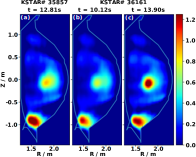
\includegraphics[width=\linewidth]{figures/Prad_2D.pdf}
 \caption{
KSTAR \ac{IRVB} measured radiated power density (a.u.) inverted into 2D cross-section.
(a) KSTAR \# 35857 at 12.81s at the peak of total radiated power.
(b) KSTAR \# 36161 at 10.12s before  the second impulse of gas between 10.8s to 12s.
(c) KSTAR \# 36161 at 13.90 after the last gas impulse.
}
\label{fig:prad_2d}
\end{figure}

Utilizing the controllers tuned in Sec.\ref{sec:sysid}, we attempted detachment control experiments.
First, we used \Afrac{} controller in KSTAR \#35857 with results shown in Fig.\ref{fig:detctrl_afrac}.
As can be seen in Fig.\ref{fig:detctrl_afrac}a, the strike point remained within 12.5~mm of one of the probes of the real-time Langmuir probe array, thus the obtained \Afrac{} signal shown in Fig.\ref{fig:detctrl_afrac}b has error $\lesssim$13\%.
Here, we can see that the controller was successful in closely following the target provided to it completing the pre-programmed shot length to the end.
It is also evident that the aggressive control strategy was reasonable in that it provided a quick response to the initial change in the target value.
There are signs of small decaying oscillations which is a characteristic of a PID loop tuned for faster-than-critical response to reach the target quickly while causing minor decaying oscillations.
While the PID loop can be made less aggressive to critically approach the target, this generally comes at the cost of approximately half the speed with which it is possible to aggressively approach the target while remaining stable.
Here we chose to demonstrate an aggressive strategy but a slower strategy without any oscillations is also possible.
From 8~s to 10~s, it can be seen that the injected N$_2$ was just enough to ramp down the measured \Afrac{} with the same slope.
The accumulated offset from the target eventually caused the integral term to send a brief impulse of nitrogen near 9.8~s and then the controller further converged with the target value.
For the rest of the shot, small nitrogen puffs were required to correct the drifting \Afrac{} and keep it on the target.
The total radiated power from the plasma as measured by KSTAR \ac{IRVB} remained below 3.5~MW ($\approx$65\% of injected power) and as can be seen in Fig.\ref{fig:prad_2d}a (snapshot taken at around the time of maximum radiation), there is a prominent concentration of radiation near the X-point.

Since \Afrac{} controller has been demonstrated in the past as well, we decided to utilize the remaining allotted runtime on KSTAR to test the DivControlNN prototype-based controller.
Fig.\ref{fig:detctrl_sm} shows the results from shot \#36161 where we deployed this controller.
An immediate issue was seen with DivControlNN output that the initial heat flux calculation had a different starting value than what we saw in reference shots and system identification shot \#35854 (this shot appeared in figures~\ref{fig:sysid_sm} and \ref{fig:SM_inputs_35854}).
Because of this, when the controller turned on at 7.5~s, the large error resulted in the railing of gas command output which caused too much N$_2$ injected into the system.
While this quickly brought down the measured signal, it also resulted in an overshoot.
In the next ramp-down of the target from 10.5~s to 11.5~s, more impurity was injected as we tuned an aggressive controller.
It can be seen from \Afrac{} in Fig.\ref{fig:detctrl_sm}d that the system reached deep detachment by this point and the ion saturation current measurements (Fig.\ref{fig:detctrl_sm}a) were in the range where low sensitivity to further evolution would be expected beyond 12~s.
Increases in core radiated power seen in \ref{fig:detctrl_sm}(e) may indicate a change in core plasma state from which recovery is not observed, as core $P_{rad}$ does not decrease later.
The decrease in power being conducted across the last closed flux surface does not help the controller follow the target back to higher heat flux, although the change in $P_{rad,core}$ is not so severe as to fully explain this.

\begin{figure*}[!ht]
\includegraphics[width=\linewidth]{figures/elm_exam_36161.pdf}
\caption{Changes in ELM properties during progression into deep detachment. Top row: D$_\alpha$ light emission, which spikes up during an ELM. Middle row: $A_{frac}$. Bottom row: Nitrogen gas command. A long time history is shown in the left column, and the four other columns zoom in at key times to show samples of individual ELMs.}
\label{fig:elms}
\end{figure*}

The failure to reattach and other behavior after reaching deepest detachment at around 12~s in \#36161 is likely due to a combination of nitrogen wall loading and changes to the ELM cycle.
Clean walls are effective at pumping nitrogen as it sticks to them, but heavily saturated walls release nitrogen and can act as a source after gas flow is turned off.
Even if the walls are only a weak or negligible source, they will be much less effective at particle removal and thus nitrogen inventory will not decrease quickly enough to follow a reattaching control target.
Inefficient pumping compared to puffing is a known challenge to control that relies on gas as the primary actuator \cite{Eldon_2017_NF,eldon_2025_ppcf}.
This type of nonlinear response also increases the risk of running an aggressive controller as periods of excess seeding may be difficult to recover from; tuning choices that could be preferable in other contexts are not necessarily the best for detachment control.
In addition to pumping issues, figure~\ref{fig:elms} shows that progression into deeper detachment is associated with changes in ELM properties.
The figure shows four time windows of equal length which are color coded;
red: prior to seeding with relatively large ELMs,
magenta: at moderate ($A_{frac} \approx 0.3$) detachment with smaller but more frequent ELMs,
blue: at deepest detachment with very weak and infrequent ELMs,
and green: after slight recovery with ELMs approaching the size seen in the magenta window.
The last two windows align with times shown in figure~\ref{fig:prad_2d}(b) and (c).
The weak ELMs at 12~s represent loss of impurity flushing across the pedestal, which is consistent with core impurity accumulation seen in figures~\ref{fig:prad_2d}(c) and \ref{fig:detctrl_sm}(e).

\begin{figure}
\centering
\includegraphics[width=\linewidth]{figures/correlation_smq_afrac.pdf}
\caption{DivControlNN heat flux versus $A_{frac}$ (a) and $n_e$ (b).
$A_{frac}$ has been renormalized to use the same correction coefficient in all cases.
The top legend gives Pearson $r$ values for each shot individually.
When all the data shown in panel (a) are aggregated, they have $r=0.62$.
Times are from 6.2~s to the end of each shot.
\#35854 was a feedforward system ID shot and \#36159 was unseeded; the others used detachment control.
}
\label{fig:correlation}
\end{figure}

Post-shot data analysis discovered further issues in our operation of the DivControlNN model.
The impurity fraction calculation as mentioned in Sec.\ref{sec:control_variables} malfunctioned and sent a constant zero input to the model (see Fig.\ref{fig:SM_inputs_35854}e).
Thus the model was unable to respond directly to large amounts of impurity that were injected into the system and was only relying on data from line-integrated core electron density, input power, and plasma current as real-time inputs.
Figure~\ref{fig:correlation}(a) shows the correlation between $A_{frac}$ and DivControlNN heat flux, showing that indeed the lowest heat flux values go with the lowest $A_{frac}$, and the highest heat flux samples are the most attached.
In the middle, however, there is an awkward step-like quality which may have been perceptible in figure~\ref{fig:detctrl_sm}(b).
This is explained by the relationship between predicted heat flux and input density in figure~\ref{fig:correlation}(b) as two regions of insensitivity to $n_e$ are apparent from about $n_e=$ 2.85--3.05 and 3.50--3.85.
Panel (b) also has a secondary curve below the primary sequence; these samples occurred at lower input power which occurred since some heating sources were not maintained until the end of every discharge.
The approximate alignment of one of the low power segments with the primary sequence section from $n_e=$ 3.05--3.50 is coincidental.
The regions of insensitivity are not desirable in a control variable and probably caused the most trouble when the DivControlNN target was set close to just below 6 from $t=11.5$--13~s in \#36161; in particular, encounter with the insensitivity from 11.5--12~s lead to an inappropriate excess in the gas command and subsequent overshooting when the heat flux output began to decrease again.
The insensitive regions reflect features observed in the UEDGE database and are being investigated.
If this is not resolved within UEDGE or within the neural network itself, an added layer could be added to eliminate these artifacts before the predicted heat flux reaches a controller.
Despite these limitations, this preliminary tests were able to regulate detachment as confirmed by the probes, and the limitations themselves highlight issues to watch for in subsequent iterations of DivControlNN or when constructing related tools.

\begin{figure*}[!ht]
\centering
\includegraphics[width=\textwidth]{figures/beta_vs_dod.pdf}
\caption{
Normalized $\beta$ plotted versus degree of detachment $DOD=1/A_{frac}$.
$A_{frac}$ has been renormalized so that all shots have the same empirical correction factor.
For seeded shots, the time range is from $t=6.0$~s until $I_p$ begins to drop.
For unseeded shots, values are averaged over $6.0<t<8.0$~s.
Vertical lines are placed as guides at $DOD = 1, 2, 5$, and 9, corresponding to guides and the axis limit of figure 12 of \cite{Eldon_2022_PPCF}.
Horizontal black lines mark typical $\beta_N$ values of attached shots in this scenario as well as various levels of degradation (see legend).
Unseeded shots are marked by opaque diamonds giving their average values over a period of steady performance during the $I_p$ flattop.
}
\label{fig:beta_vs_dod}
\end{figure*}

Figure~\ref{fig:beta_vs_dod} shows how detachment with nitrogen seeding affects core plasma performance.
As this scenario is based on the previous scenario used with the carbon divertor, trends are similar: 20\% drop in $\beta_N$ at $DOD\approx 5$ and 30\% drop at $DOD\sim 9$ compared to the average $\beta_N$ value for unseeded shots.
However, the initial loss of $\beta$ at $DOD\approx 2$ is greater at $\approx 15$\% in these recent shots in the tungsten vertical divertor compared to $\approx 10$\% for nitrogen-seeded shots at $DOD=2$ in the carbon central-slant divertor.
We note that detachment control with deuterium in the carbon divertor resulted in $\beta_N$ dropping in $\approx 15$--$20$\% at $DOD=2$, and attribute this faster initial drop to deuterium puffing as a less efficient actuator for detachment than impurity seeding.
Perhaps lack of a local carbon sputtering source at the strike point requires more nitrogen be added to initiate detachment, but deeper detachment levels are similar as both cases (C and W divertors) have nitrogen as the dominant impurity by then, and also sputtering of carbon at the strike point will be reduced by detachment.
The general trend of performance changes during detachment seems to be dominated by the core scenario, as seen in figure~5 of \cite{wang_2021_pop}.
Isolated detachment control systems like the ones presented here primarily control motion along the $\beta$ vs $DOD$ curves set by the scenario, although some hysteresis is evident in the discharges that used feed-forward control (magenta and purple).
In \#35853, returning from $DOD>10$ to $DOD\sim5$ did not proceed along the original curve, but instead some permanent loss of $\beta$ occurred.
A simple, single-in, single-out controller (SISO), if properly configured, should be able to prevent deleterious changes to the core scenario like this by avoiding unnecessarily deep detachment and over seeding.
SISO controllers were used to control detachment in the high $\beta_p$ scenario shown in \cite{wang_2021_pop} figure~5, and consistent with the trends shown in that figure, they delivered deep detachment without confinement degradation (but with a problematic level of fuel dilution) \cite{Eldon_2021_NME}.
It may be possible for an isolated detachment controller to change the $\beta$ vs $DOD$ curve by injeting fuel in addition to an impurity species in a single-in, multi-out scheme.
This strategy may be able to increase the dissipation efficiency of the seeded impurity and reduce fuel dilution and undesirable side effects of impurity-induced detachment because $P_{rad}=n_e n_Z L_Z(T_e)$: impurity density $n_Z$ is not the only tool at our disposal.


\section{Discussion}
\label{sec:discussion}

In this paper, we described re-using \Afrac as a reliable control variable for detachment control provided that real-time ion saturation current measurements are available from the Langmuir probes and the strike point is controlled well enough that such an array can be used to estimate peak $I_{sat}$.
It can be seen from panels (a) and (c) in Fig.\ref{fig:sysid_afrac}, Fig.\ref{fig:sysid_sm}, and Fig.\ref{fig:detctrl_sm} that when the total injected impurity amount crosses a rough threshold of about $1\times10^{20}$ particles, the plasma boundary shape is deformed such that strike point on outer divertor starts drifting downwards (and the inner strike point moves upwards) even though the X-point is held in place by the magnetic shape control system.
% This change in divertor leg angle and corresponding changes to the rest of the nearby boundary is sometimes described as rotation of the boundary about the X-point.  % I don't think you need this but IDK.
Thus, \Afrac controller is best suited with an outer strike point control system commissioned on the device, as was demonstrated in the previous carbon divertor \cite{Eldon_2022_PPCF}.
Unfortunately, direct strike point position control (rather than X-point position control), was not yet commissioned for the new divertor at the time of these tests.
It is also important to keep note of the position of strike point and the width of the ion saturation current profile on the divertor.
In our case, we estimated that the ion saturation current profile width is about 16~mm, just enough to ensure that at least one of the Langmuir probes is always inside the wetted area from the \ac{SOL} plasma.
% \textcolor{red}{The strike \emph{point} has no width. The Isat profile has a FWHM of $\approx$16~mm. Other vocabulary that can be used in general situations similar to this are things like profiles at the divertor target plate, Jsat distributions, downstream Jsat, divertor profiles, etc. Comparing the Isat or Jsat profile to the probe spacing puts an upper bound on error in estimating the peak Jsat due to bad alignment between probes and strike point. BTW the pitch angle of the field changes across the plate so the probes don't have the same effective area normal to the magnetic field, even if they have the same physical dimensions. So the Jsat profile could be deformed a little compared to the Isat profile. If the X-point is close to the target, the deformation will be more severe. The probes near the strike point will tend to have lower effective area (although exceptions can be created with weird shapes on flexible devices like d3d and tcv) since the poloidal field is weaker near the X-point. This will probably make the Jsat have a sharper peak than Isat. And Jsat is more intrinsic to the plasma. You don't have to write any of this; just don't think that Isatprofile = Jsatprofile * constant.}
Even then, it can be seen that at around 12.4s in Fig.\ref{fig:sysid_afrac} and at around 10s in Fig.\ref{fig:detctrl_afrac} that as the strike point moves from OD9 (Z=-1.225m) to OD11(Z=-1.2125m), the corresponding \Afrac value shows a sharp decline and then recovery, probably due to the peak passing through the middle of the two probes.
This effect is small enough that our existing controller was able to fix it, but it shows a potential source of error in system identification and might also cause loss of control if the sudden transition can excite an unstable oscillation of the \ac{UGF}.
For future applications of this controller, we are working on including real-time spatial analysis of the $J_{sat}$ profile, potentially informed with profile shapes from high-fidelity simulations from SOLPS-ITER or UEDGE.

In our experimental session, since strike point control had not been commissioned, we attempted real-time empirical profile analysis with strike point sweeps.
But we found that the actuation strength and response time of the poloidal field coils at KSTAR do not allow for large enough and fast enough strike point sweeps.
% \textcolor{red}{Do you want to mention that we attempted real-time empirical profile analysis with strike point sweeps, but found that KSTAR's coils could make big+fast enough sweeps? This would probably work at d3d, but now who cares because it won't work in the long pulse devices. I am in favor of documenting good ideas that don't work so others don't try them without expanding them to solve the issues we found. It also shows we prepared/tried to prepare for a lot of possible gotchas. Things got weird but we really did think a lot of things through in our designs.}

It should be noted that in the application of \Afrac controller method on KSTAR, tuning the overall factor to \Afrac so that it reports 1.0 when fully attached was trickier than the case for full carbon environment KSTAR \cite{Eldon_2022_PPCF}.
We noticed offsets in the outputs of Langmuir probes which changed from shot to shot, and thus ensuring the correct normalizing factor for \Afrac became harder.
This was the reason why we had to change the factor for \Afrac after shot \#35853 as also mentioned in the caption of Fig.\ref{fig:sysid_afrac}.
After this experience, we have now added an online offset estimator and subtraction for all probe signals, which measures the offset before the plasma breakdown and ensures that the zero offset is correct on the probes.
This issue is likely due to electrical connectivity problems with the probes which also showed other issues during the campaign, but still, this experience should be noted for future reproduction and improvements.

Another point of uncertainty in \Afrac model could be the magnetic connection length between the upstream (outboard midplane) and divertor in the 2PM \cite{Leonard_2018_PPCF}.
This length is kept fixed in the model and while we did not change the plasma boundary shape much from the previous test \cite{Eldon_2022_PPCF} in carbon divertor KSTAR, it still makes it a potential source of error in wider usage in future.
The real-time equilibrium calculations during shot provided by RTEFIT is being upgraded to also output this magnetic connection length so that in future the model gets more accurate and time varying information about this important parameter.
% \textcolor{red}{The magnetic connection length between the upstream (outboard midplane) and divertor in the TPM is one of the important inputs, but it would've changed as we tried to optimize the shape. I think this could've been part of the problems. In carbon, I used a shape that had been dialed in pretty well thanks to colleagues like Junghoo Hwang and Matthias Bernert, and the preliminary sys ID shots I took. In tungsten, we were trying to do many changes at once to keep the scenario together. We are doing an upgrade to have RTEFIT output this connection length $L_\parallel$ so that we won't have to recalibrate this aspect of the model during shape changes.}

Although Langmuir probes might not be able to survive future burning plasma experiments, they are still a valuable tool for studying detachment control experiments for ease of installation and operation in experimental devices.
Even in burning plasma devices, sacrificial Langmuir probes can be used in initial device commissioning and preparation of base scenarios at low power, although they are expected to fail shortly after exposure to the intensity of full heat and neutron fluxes.
Knowing what a stable detached scenario should be like could significantly decrease the time required to commission controllers based on other control variables, and give a baseline level of detachment control performance to compare them to.
Thus, Langmuir probe based control might provide a foothold in future device commissioning, as it has been shown to be useful on many devices \cite{Eldon_2021_NME, Guillemaut_2017_PPCF, Yuan_2020_FED, Khodunov_2021_PPCF}.
The good results from \Afrac controller as seen in Fig.\ref{fig:detctrl_afrac} could also motivate further research in similar biased electrode measurement methods of SOL plasma such as biased divertor plates \cite{Toi_2023_NF, Cui_2024_NF} which behave like larger area Langmuir probes and can withstand harsher conditions in comparison to small tip area probes.

We also demonstrated using a machine-learning-based surrogate model, DivControlNN, which infers from a large database of 2D UEDGE simulations for estimating hard to infer quantities in the plasma, such as heat flux on the divertor, for controlling detachment level with real-time feedback.
% \textcolor{red}{KSTAR did have IR thermography for heat flux before; not sure if it works in tungsten but be careful with calling heat flux inaccessible. Might want to rephrase.}
As of the writing of this manuscript, this detachment control method is the first of its kind ever implemented and will act as a stepping stone for future deployments.
This is an important step in the direction of achieving detachment control in future burning plasma reactors which would have very limited means of measuring the detachment level due to space constraints and harsh environment.

We have identified critical weak points in the prototype of DivControlNN and the control infrastructure required to utilize this model, and we are working on improving these aspects for future tests.
One likely mistake we made during the experiments was treating the long dead time reported by DivControlNN heat flux output in response to gas puff (Fig.\ref{fig:sysid_sm}) as an overestimate.
Since DivControlNN had a constant zero impurity fraction concentration, it was solely relying on line integrated core electron density information for responding to changes.
While ion saturation currents provide local divertor information fast, the core electron density response to gas puff would have additional transport timescales and thus DivControlNN output might truly have a larger daed time.
This could have resulted in the high controller gain that saturated the gas response in the test (Fig.\ref{fig:detctrl_sm}).

We are in the process of creating a new 2D UEDGE database of KSTAR with a tungsten divertor and considering multiple charged states of additional impurities such as nitrogen, neon, and argon.
New models would be trained on the expanded database and acquired experimental data from this campaign, with the input of injected gas flow instead of impurity fraction to simplify the use case of these models.
We would also work with the KSTAR team to improve PCS communication infrastructure so that accurate real-time values of injected power are available to our models.

The initial success of the neural network surrogate model in detachment control motivates and corroborates similar studies, simulations, and training of other models for providing fast estimates of plasma parameters, for quick decision-making in the control room during experiments, as well as, for potential use in other control systems where important plasma properties are often not accessible directly.
A neural network based control system approach has already been demonstrated in magnetic shape control \cite{Degrave_2022_Nature}.
For \ac{SOL} plasma predictions, machine learning surrogate models were first pioneered using 1D UEDGE simulations \cite{Zhu_2022_JPP}, serving as the proof-of-principle study that paved the way for DivControlNN presented here, which is based on 2D UEDGE simulations.
More recently, model based on Hermes-3 \cite{Dudson_2024_CPC} simulations of MAST-U \cite{Holt_2024_NF} and neural partial differential equation solver for TCV \cite{Poels_2023_NF} have been reported and are under further development.

Another major focus of future experiments would be to use noble gases in detachment control.
N$_2$, while being excellent at cooling the SOL plasma in conventional tokamaks, would not be a good impurity to seed in tritium fueled plasma due to the formation of tritiated ammonia \cite{Pitts_2019_NME}.
Such tritiated ammonia would require additional tritium reclaiming processes which would reduce the duty cycle of reactors, as well as, pose additional risks in handling a radioactive gas.
% \textcolor{red}{Check whether it's actually more dangerous than any other tritium contamination or just much harder to process to reclaim the precious tritium. And yes, more tritium processing is more opportunity for something to go wrong, so technically it might increase the danger level, but this isn't necessarily by a lot. Is that really significant? I would check to be sure before talking about danger.}
We are in the process of testing Ne and Ar as alternate cooling gases.
In the KSTAR scenarios investigated so far, the effect of Ne on detachment has been hard to observe as small gas puffs do not actuate enough on the \ac{SOL} plasma but if the gas puffing is increased, we suddenly observe disruption due to too much cooling inside the separatrix.
% Commenting out the following for now. Verifying this.
% More widely, there has been recent interest in using pellets for impurity injection for detachment control to reduce the large lag time and response time associated with gas puffing.
% Another alternative is dropping the impurity in the form of solid powder, such as Boron.
% However, the investigation on its use for this purpose is still in a preliminary phase and poses additional challenges in terms of long lag time due to free fall and accumulation of unused powder in the device.
% \textcolor{red}{Who's doing impurity pellets? The disruption mitigation ones don't count.} 


\section*{CRediT authorship contribution statement}

\textbf{A.~Gupta} conceptualization,  methodology, software, formal analysis, data curation, visualization, writing - original draft.
\textbf{D.~Eldon} conceptualization, methodology, software, writing - review \& editing, supervision, funding acquisition.
\textbf{H.~Anand} resources.
\textbf{A.~Dautt-Silva} software, resources.
\textbf{S.~De Pascuale} conceptualization, software
\textbf{J.~Lore} conceptualization, software, data curation, funding acquisition.
\textbf{O.~Meneghini} methodology, software.
\textbf{J.-S.~Park} conceptualization, software, data curation.

\input{sections/declaration_of_competing_interest}

\section*{Acknowledgements}

Special thanks to Anthony Leonard for his guidance and useful discussion on this work.

This material is based upon work supported by the U.S. Department of Energy, Office of Science, Office of Fusion Energy Sciences under the Spherical Tokamak program,
% using the DIII-D National Fusion Facility, a DOE Office of Science user facility,
under Awards 
DE-FC02-04ER54698,  % General DIII-D / GA & ORAU  (checked 2024-03-08)
% DE-SC002340, % KSTAR detachment control / GA (current through 2025-08-31; may change at renewal)
DE-SC0023250 % SPARC heat flux control / GA (current through 2025-08-31; may change at renewal)
and
DE-AC05-00OR22725. % SPARC heat flux control / ORNL (current through 2025-08-31; may change at renewal)
% DE-AC52-07NA27344,  % DIII-D / LLNL (current: doesn't change)
% and
% DE-NA0003525.  % DIII-D / SNL (current: doesn't change)

% From https://fusionga.sharepoint.com/sites/DIII-DHub/SitePages/Acknowledgements-Required-for-Research-Products.aspx :
%The national laboratory contract numbers for DIII-D work do not change, and are not listed in PAMS (because they are not awards). The relevant contract numbers are, 
%Princeton Plasma Physics Laboratory: DE-AC02-09CH11466
%Oak Ridge National Laboratory: DE-AC05-00OR22725
%Lawrence Livermore National Laboratory:  DE-AC52-07NA27344
%Sandia National Laboratory: DE-NA0003525
%Argonne National Laboratory: DE-AC02-06CH11357

\input{sections/disclaimer}

\bibliography{refs}

\end{document}
